\title{Restricciones de Dominio para Cada Columna}

\maketitle

\section*{1. Tabla: \texttt{Pais}}
\begin{itemize}
    \item \texttt{NombrePais}: \texttt{varchar(50) NOT NULL} 
    \begin{itemize}
        \item Restricción: No puede ser nulo. Clave primaria.
    \end{itemize}
\end{itemize}

\section*{2. Tabla: \texttt{Medallero}}
\begin{itemize}
    \item \texttt{IDMedallero}: \texttt{serial PRIMARY KEY} 
    \begin{itemize}
        \item Restricción: Clave primaria generada automáticamente.
    \end{itemize}
    \item \texttt{NombrePais}: \texttt{varchar(50)} 
    \begin{itemize}
        \item Restricción: Referencia a \texttt{Pais} (clave foránea).
    \end{itemize}
\end{itemize}

\section*{3. Tabla: \texttt{Gana}}
\begin{itemize}
    \item \texttt{NombrePais}: \texttt{varchar(50) NOT NULL}
    \begin{itemize}
        \item Restricción: No puede ser nulo, clave foránea.
    \end{itemize}
    \item \texttt{TipoMedalla}: \texttt{varchar(10)}
    \begin{itemize}
        \item Restricción: Longitud máxima de 10 caracteres, clave foránea.
    \end{itemize}
    \item \texttt{IDDisciplina}: \texttt{int}
    \begin{itemize}
        \item Restricción: Clave foránea.
    \end{itemize}
    \item \textbf{PRIMARY KEY}: (\texttt{NombrePais}, \texttt{TipoMedalla}, \texttt{IDDisciplina}).
\end{itemize}

\section*{4. Tabla: \texttt{Concursa}}
\begin{itemize}
    \item \texttt{IDAtleta}: \texttt{int NOT NULL}
    \begin{itemize}
        \item Restricción: No puede ser nulo, clave foránea.
    \end{itemize}
    \item \texttt{IDEvento}: \texttt{int NOT NULL}
    \begin{itemize}
        \item Restricción: No puede ser nulo, clave foránea.
    \end{itemize}
    \item \textbf{PRIMARY KEY}: (\texttt{IDAtleta}, \texttt{IDEvento}).
\end{itemize}

\section*{5. Tabla: \texttt{TelefonoAtleta}}
\begin{itemize}
    \item \texttt{IDTelefono}: \texttt{int NOT NULL}
    \begin{itemize}
        \item Restricción: No puede ser nulo, clave primaria.
    \end{itemize}
    \item \texttt{IDAtleta}: \texttt{int}
    \begin{itemize}
        \item Restricción: Clave foránea.
    \end{itemize}
\end{itemize}

\section*{6. Tabla: \texttt{CorreoAtleta}}
\begin{itemize}
    \item \texttt{IDCorreo}: \texttt{varchar(50) NOT NULL}
    \begin{itemize}
        \item Restricción: Longitud máxima de 50 caracteres, clave primaria.
    \end{itemize}
    \item \texttt{IDAtleta}: \texttt{int}
    \begin{itemize}
        \item Restricción: Clave foránea.
    \end{itemize}
\end{itemize}

\section*{7. Tabla: \texttt{Atleta}}
\begin{itemize}
    \item \texttt{IDAtleta}: \texttt{serial PRIMARY KEY}
    \begin{itemize}
        \item Restricción: Clave primaria generada automáticamente.
    \end{itemize}
    \item \texttt{NombrePais}: \texttt{varchar(50)}
    \begin{itemize}
        \item Restricción: Clave foránea.
    \end{itemize}
    \item \texttt{IDEntrenador}: \texttt{int}
    \begin{itemize}
        \item Restricción: Clave foránea.
    \end{itemize}
    \item \texttt{Temporada}: \texttt{date default now()}
    \begin{itemize}
        \item Restricción: Fecha, valor por defecto es la fecha actual.
    \end{itemize}
    \item \texttt{Nombre}: \texttt{varchar(50) NOT NULL}
    \begin{itemize}
        \item Restricción: Longitud máxima de 50 caracteres, no puede ser nulo.
    \end{itemize}
    \item \texttt{PrimerApellido}: \texttt{varchar(50) default 'No proporcionado'}
    \begin{itemize}
        \item Restricción: Longitud máxima de 50 caracteres, valor por defecto es 'No proporcionado'.
    \end{itemize}
    \item \texttt{SegundoApellido}: \texttt{varchar(50) default 'No proporcionado'}
    \begin{itemize}
        \item Restricción: Longitud máxima de 50 caracteres, valor por defecto es 'No proporcionado'.
    \end{itemize}
    \item \texttt{FechaNacimiento}: \texttt{date NOT NULL}
    \begin{itemize}
        \item Restricción: No puede ser nulo.
    \end{itemize}
    \item \texttt{Nacionalidad}: \texttt{varchar(50) default 'No proporcionado'}
    \begin{itemize}
        \item Restricción: Longitud máxima de 50 caracteres, valor por defecto es 'No proporcionado'.
    \end{itemize}
    \item \texttt{Genero}: \texttt{char(1) default 0}
    \begin{itemize}
        \item Restricción: Un solo carácter, valor por defecto es 0.
    \end{itemize}
\end{itemize}

\section*{8. Tabla: \texttt{Participa}}
\begin{itemize}
    \item \texttt{IDAtleta}: \texttt{int NOT NULL}
    \begin{itemize}
        \item Restricción: No puede ser nulo, clave foránea.
    \end{itemize}
    \item \texttt{IDDisciplina}: \texttt{int NOT NULL}
    \begin{itemize}
        \item Restricción: No puede ser nulo, clave foránea.
    \end{itemize}
    \item \textbf{PRIMARY KEY}: (\texttt{IDAtleta}, \texttt{IDDisciplina}).
\end{itemize}

\section*{9. Tabla: \texttt{Medalla}}
\begin{itemize}
    \item \texttt{TipoMedalla}: \texttt{varchar(10) NOT NULL}
    \begin{itemize}
        \item Restricción: Longitud máxima de 10 caracteres, no puede ser nulo.
    \end{itemize}
    \item \texttt{IDDisciplina}: \texttt{int NOT NULL}
    \begin{itemize}
        \item Restricción: No puede ser nulo, clave foránea.
    \end{itemize}
    \item \textbf{PRIMARY KEY}: (\texttt{TipoMedalla}, \texttt{IDDisciplina}).
\end{itemize}

\section*{10. Tabla: \texttt{Evento}}
\begin{itemize}
    \item \texttt{IDEvento}: \texttt{serial PRIMARY KEY}
    \begin{itemize}
        \item Restricción: Clave primaria generada automáticamente.
    \end{itemize}
    \item \texttt{NombreLocalidad}: \texttt{varchar(50)}
    \begin{itemize}
        \item Restricción: Clave foránea.
    \end{itemize}
    \item \texttt{IDDisciplina}: \texttt{int}
    \begin{itemize}
        \item Restricción: Clave foránea.
    \end{itemize}
    \item \texttt{DuracionMax}: \texttt{int NOT NULL}
    \begin{itemize}
        \item Restricción: No puede ser nulo.
    \end{itemize}
    \item \texttt{Precio}: \texttt{int NOT NULL}
    \begin{itemize}
        \item Restricción: No puede ser nulo.
    \end{itemize}
    \item \texttt{FechaEvento}: \texttt{date NOT NULL}
    \begin{itemize}
        \item Restricción: No puede ser nulo.
    \end{itemize}
    \item \texttt{Fase}: \texttt{int default 0}
    \begin{itemize}
        \item Restricción: Valor entero, valor por defecto es 0.
    \end{itemize}
\end{itemize}

\section*{11. Tabla: \texttt{TelefonoEntrenador}}
\begin{itemize}
    \item \texttt{IDTelefono}: \texttt{int NOT NULL}
    \begin{itemize}
        \item Restricción: No puede ser nulo, clave primaria.
    \end{itemize}
    \item \texttt{IDEntrenador}: \texttt{int}
    \begin{itemize}
        \item Restricción: Clave foránea.
    \end{itemize}
\end{itemize}

\section*{12. Tabla: \texttt{Disciplina}}
\begin{itemize}
    \item \texttt{IDDisciplina}: \texttt{serial PRIMARY KEY}
    \begin{itemize}
        \item Restricción: Clave primaria generada automáticamente.
    \end{itemize}
    \item \texttt{NombreDisciplina}: \texttt{varchar(50) NOT NULL}
    \begin{itemize}
        \item Restricción: Longitud máxima de 50 caracteres, no puede ser nulo.
    \end{itemize}
    \item \texttt{Categoria}: \texttt{varchar(50) NOT NULL}
    \begin{itemize}
        \item Restricción: Longitud máxima de 50 caracteres, no puede ser nulo.
    \end{itemize}
\end{itemize}

\section*{13. Tabla: \texttt{Localidad}}
\begin{itemize}
    \item \texttt{NombreLocalidad}: \texttt{varchar(50) NOT NULL}
    \begin{itemize}
        \item Restricción: Longitud máxima de 50 caracteres, clave primaria.
    \end{itemize}
    \item \texttt{IDDisciplina}: \texttt{int NOT NULL}
    \begin{itemize}
        \item Restricción: Clave foránea, no puede ser nulo.
    \end{itemize}
    \item \texttt{Calle}: \texttt{varchar(50) NOT NULL}
    \begin{itemize}
        \item Restricción: Longitud máxima de 50 caracteres, no puede ser nulo.
    \end{itemize}
    \item \texttt{Numero}: \texttt{int NOT NULL}
    \begin{itemize}
        \item Restricción: No puede ser nulo.
    \end{itemize}
    \item \texttt{Ciudad}: \texttt{varchar(50) NOT NULL}
    \begin{itemize}
        \item Restricción: Longitud máxima de 50 caracteres, no puede ser nulo.
    \end{itemize}
    \item \texttt{Pais}: \texttt{varchar(50) NOT NULL}
    \begin{itemize}
        \item Restricción: Longitud máxima de 50 caracteres, no puede ser nulo.
    \end{itemize}
    \item \texttt{Aforo}: \texttt{int NOT NULL}
    \begin{itemize}
        \item Restricción: No puede ser nulo.
    \end{itemize}
    \item \texttt{Tipo}: \texttt{int NOT NULL}
    \begin{itemize}
        \item Restricción: No puede ser nulo.
    \end{itemize}
\end{itemize}

\section*{14. Tabla: \texttt{CompraEntrada}}
\begin{itemize}
    \item \texttt{IDCliente}: \texttt{int NOT NULL}
    \begin{itemize}
        \item Restricción: No puede ser nulo, clave foránea.
    \end{itemize}
    \item \texttt{IDEvento}: \texttt{int NOT NULL}
    \begin{itemize}
        \item Restricción: No puede ser nulo, clave foránea.
    \end{itemize}
    \item \textbf{PRIMARY KEY}: (\texttt{IDCliente}, \texttt{IDEvento}).
\end{itemize}

\section*{15. Tabla: \texttt{Cliente}}
\begin{itemize}
    \item \texttt{IDCliente}: \texttt{serial PRIMARY KEY}
    \begin{itemize}
        \item Restricción: Clave primaria generada automáticamente.
    \end{itemize}
    \item \texttt{Nombre}: \texttt{varchar(50) NOT NULL}
    \begin{itemize}
        \item Restricción: Longitud máxima de 50 caracteres, no puede ser nulo.
    \end{itemize}
    \item \texttt{Correo}: \texttt{varchar(50) NOT NULL}
    \begin{itemize}
        \item Restricción: Longitud máxima de 50 caracteres, no puede ser nulo.
    \end{itemize}
    \item \texttt{Telefono}: \texttt{varchar(10)}
    \begin{itemize}
        \item Restricción: Longitud máxima de 10 caracteres.
    \end{itemize}
\end{itemize}

\section*{16. Tabla: \texttt{CorreoEntrenador}}
\begin{itemize}
    \item \texttt{IDCorreo}: \texttt{varchar(50) NOT NULL}
    \begin{itemize}
        \item Restricción: Longitud máxima de 50 caracteres, no puede ser nulo, clave primaria.
    \end{itemize}
    \item \texttt{IDEntrenador}: \texttt{int}
    \begin{itemize}
        \item Restricción: Clave foránea.
    \end{itemize}
\end{itemize}

\section*{17. Tabla: \texttt{Entrenador}}
\begin{itemize}
    \item \texttt{IDEntrenador}: \texttt{serial PRIMARY KEY}
    \begin{itemize}
        \item Restricción: Clave primaria generada automáticamente.
    \end{itemize}
    \item \texttt{IDDisciplina}: \texttt{int}
    \begin{itemize}
        \item Restricción: Clave foránea.
    \end{itemize}
    \item \texttt{Nombre}: \texttt{varchar(50) NOT NULL}
    \begin{itemize}
        \item Restricción: Longitud máxima de 50 caracteres, no puede ser nulo.
    \end{itemize}
    \item \texttt{PrimerApellido}: \texttt{varchar(50) default 'No proporcionado'}
    \begin{itemize}
        \item Restricción: Longitud máxima de 50 caracteres, valor por defecto es 'No proporcionado'.
    \end{itemize}
    \item \texttt{SegundoApellido}: \texttt{varchar(50) default 'No proporcionado'}
    \begin{itemize}
        \item Restricción: Longitud máxima de 50 caracteres, valor por defecto es 'No proporcionado'.
    \end{itemize}
    \item \texttt{FechaNacimiento}: \texttt{date NOT NULL}
    \begin{itemize}
        \item Restricción: No puede ser nulo.
    \end{itemize}
    \item \texttt{Nacionalidad}: \texttt{varchar(50) default 'No proporcionado'}
    \begin{itemize}
        \item Restricción: Longitud máxima de 50 caracteres, valor por defecto es 'No proporcionado'.
    \end{itemize}
    \item \texttt{Genero}: \texttt{char(1) default 0}
    \begin{itemize}
        \item Restricción: Un solo carácter, valor por defecto es 0.
    \end{itemize}
\end{itemize}

\section*{18. Tabla: \texttt{TelefonoArbitro}}
\begin{itemize}
    \item \texttt{IDTelefono}: \texttt{int NOT NULL}
    \begin{itemize}
        \item Restricción: No puede ser nulo, clave primaria.
    \end{itemize}
    \item \texttt{IDArbitro}: \texttt{int}
    \begin{itemize}
        \item Restricción: Clave foránea.
    \end{itemize}
\end{itemize}

\section*{19. Tabla: \texttt{Patrocina}}
\begin{itemize}
    \item \texttt{NombrePatrocinador}: \texttt{varchar(50) NOT NULL}
    \begin{itemize}
        \item Restricción: No puede ser nulo, clave foránea.
    \end{itemize}
    \item \texttt{IDDisciplina}: \texttt{int NOT NULL}
    \begin{itemize}
        \item Restricción: No puede ser nulo, clave foránea.
    \end{itemize}
    \item \textbf{PRIMARY KEY}: (\texttt{NombrePatrocinador}, \texttt{IDDisciplina}).
\end{itemize}

\section*{20. Tabla: \texttt{Arbitro}}
\begin{itemize}
    \item \texttt{IDArbitro}: \texttt{serial PRIMARY KEY}
    \begin{itemize}
        \item Restricción: Clave primaria generada automáticamente.
    \end{itemize}
    \item \texttt{IDDisciplina}: \texttt{int}
    \begin{itemize}
        \item Restricción: Clave foránea.
    \end{itemize}
    \item \texttt{Nombre}: \texttt{varchar(50) NOT NULL}
    \begin{itemize}
        \item Restricción: Longitud máxima de 50 caracteres, no puede ser nulo.
    \end{itemize}
    \item \texttt{PrimerApellido}: \texttt{varchar(50) default 'No proporcionado'}
    \begin{itemize}
        \item Restricción: Longitud máxima de 50 caracteres, valor por defecto es 'No proporcionado'.
    \end{itemize}
    \item \texttt{SegundoApellido}: \texttt{varchar(50) default 'No proporcionado'}
    \begin{itemize}
        \item Restricción: Longitud máxima de 50 caracteres, valor por defecto es 'No proporcionado'.
    \end{itemize}
    \item \texttt{FechaNacimiento}: \texttt{date NOT NULL}
    \begin{itemize}
        \item Restricción: No puede ser nulo.
    \end{itemize}
    \item \texttt{Nacionalidad}: \texttt{varchar(50) default 'No proporcionado'}
    \begin{itemize}
        \item Restricción: Longitud máxima de 50 caracteres, valor por defecto es 'No proporcionado'.
    \end{itemize}
    \item \texttt{Genero}: \texttt{char(1) default 0}
    \begin{itemize}
        \item Restricción: Un solo carácter, valor por defecto es 0.
    \end{itemize}
\end{itemize}

\section*{21. Tabla: \texttt{CorreoArbitro}}
\begin{itemize}
    \item \texttt{IDCorreo}: \texttt{varchar(50) NOT NULL}
    \begin{itemize}
        \item Restricción: Longitud máxima de 50 caracteres, clave primaria.
    \end{itemize}
    \item \texttt{IDArbitro}: \texttt{int}
    \begin{itemize}
        \item Restricción: Clave foránea.
    \end{itemize}
\end{itemize}

\section*{22. Tabla: \texttt{Patrocinador}}
\begin{itemize}
    \item \texttt{NombrePatrocinador}: \texttt{varchar(50) NOT NULL}
    \begin{itemize}
        \item Restricción: Longitud máxima de 50 caracteres, clave primaria.
    \end{itemize}
\end{itemize}


\section{Modelo Relacional de la Práctica 4:}
\begin{figure}[h]
    \centering
    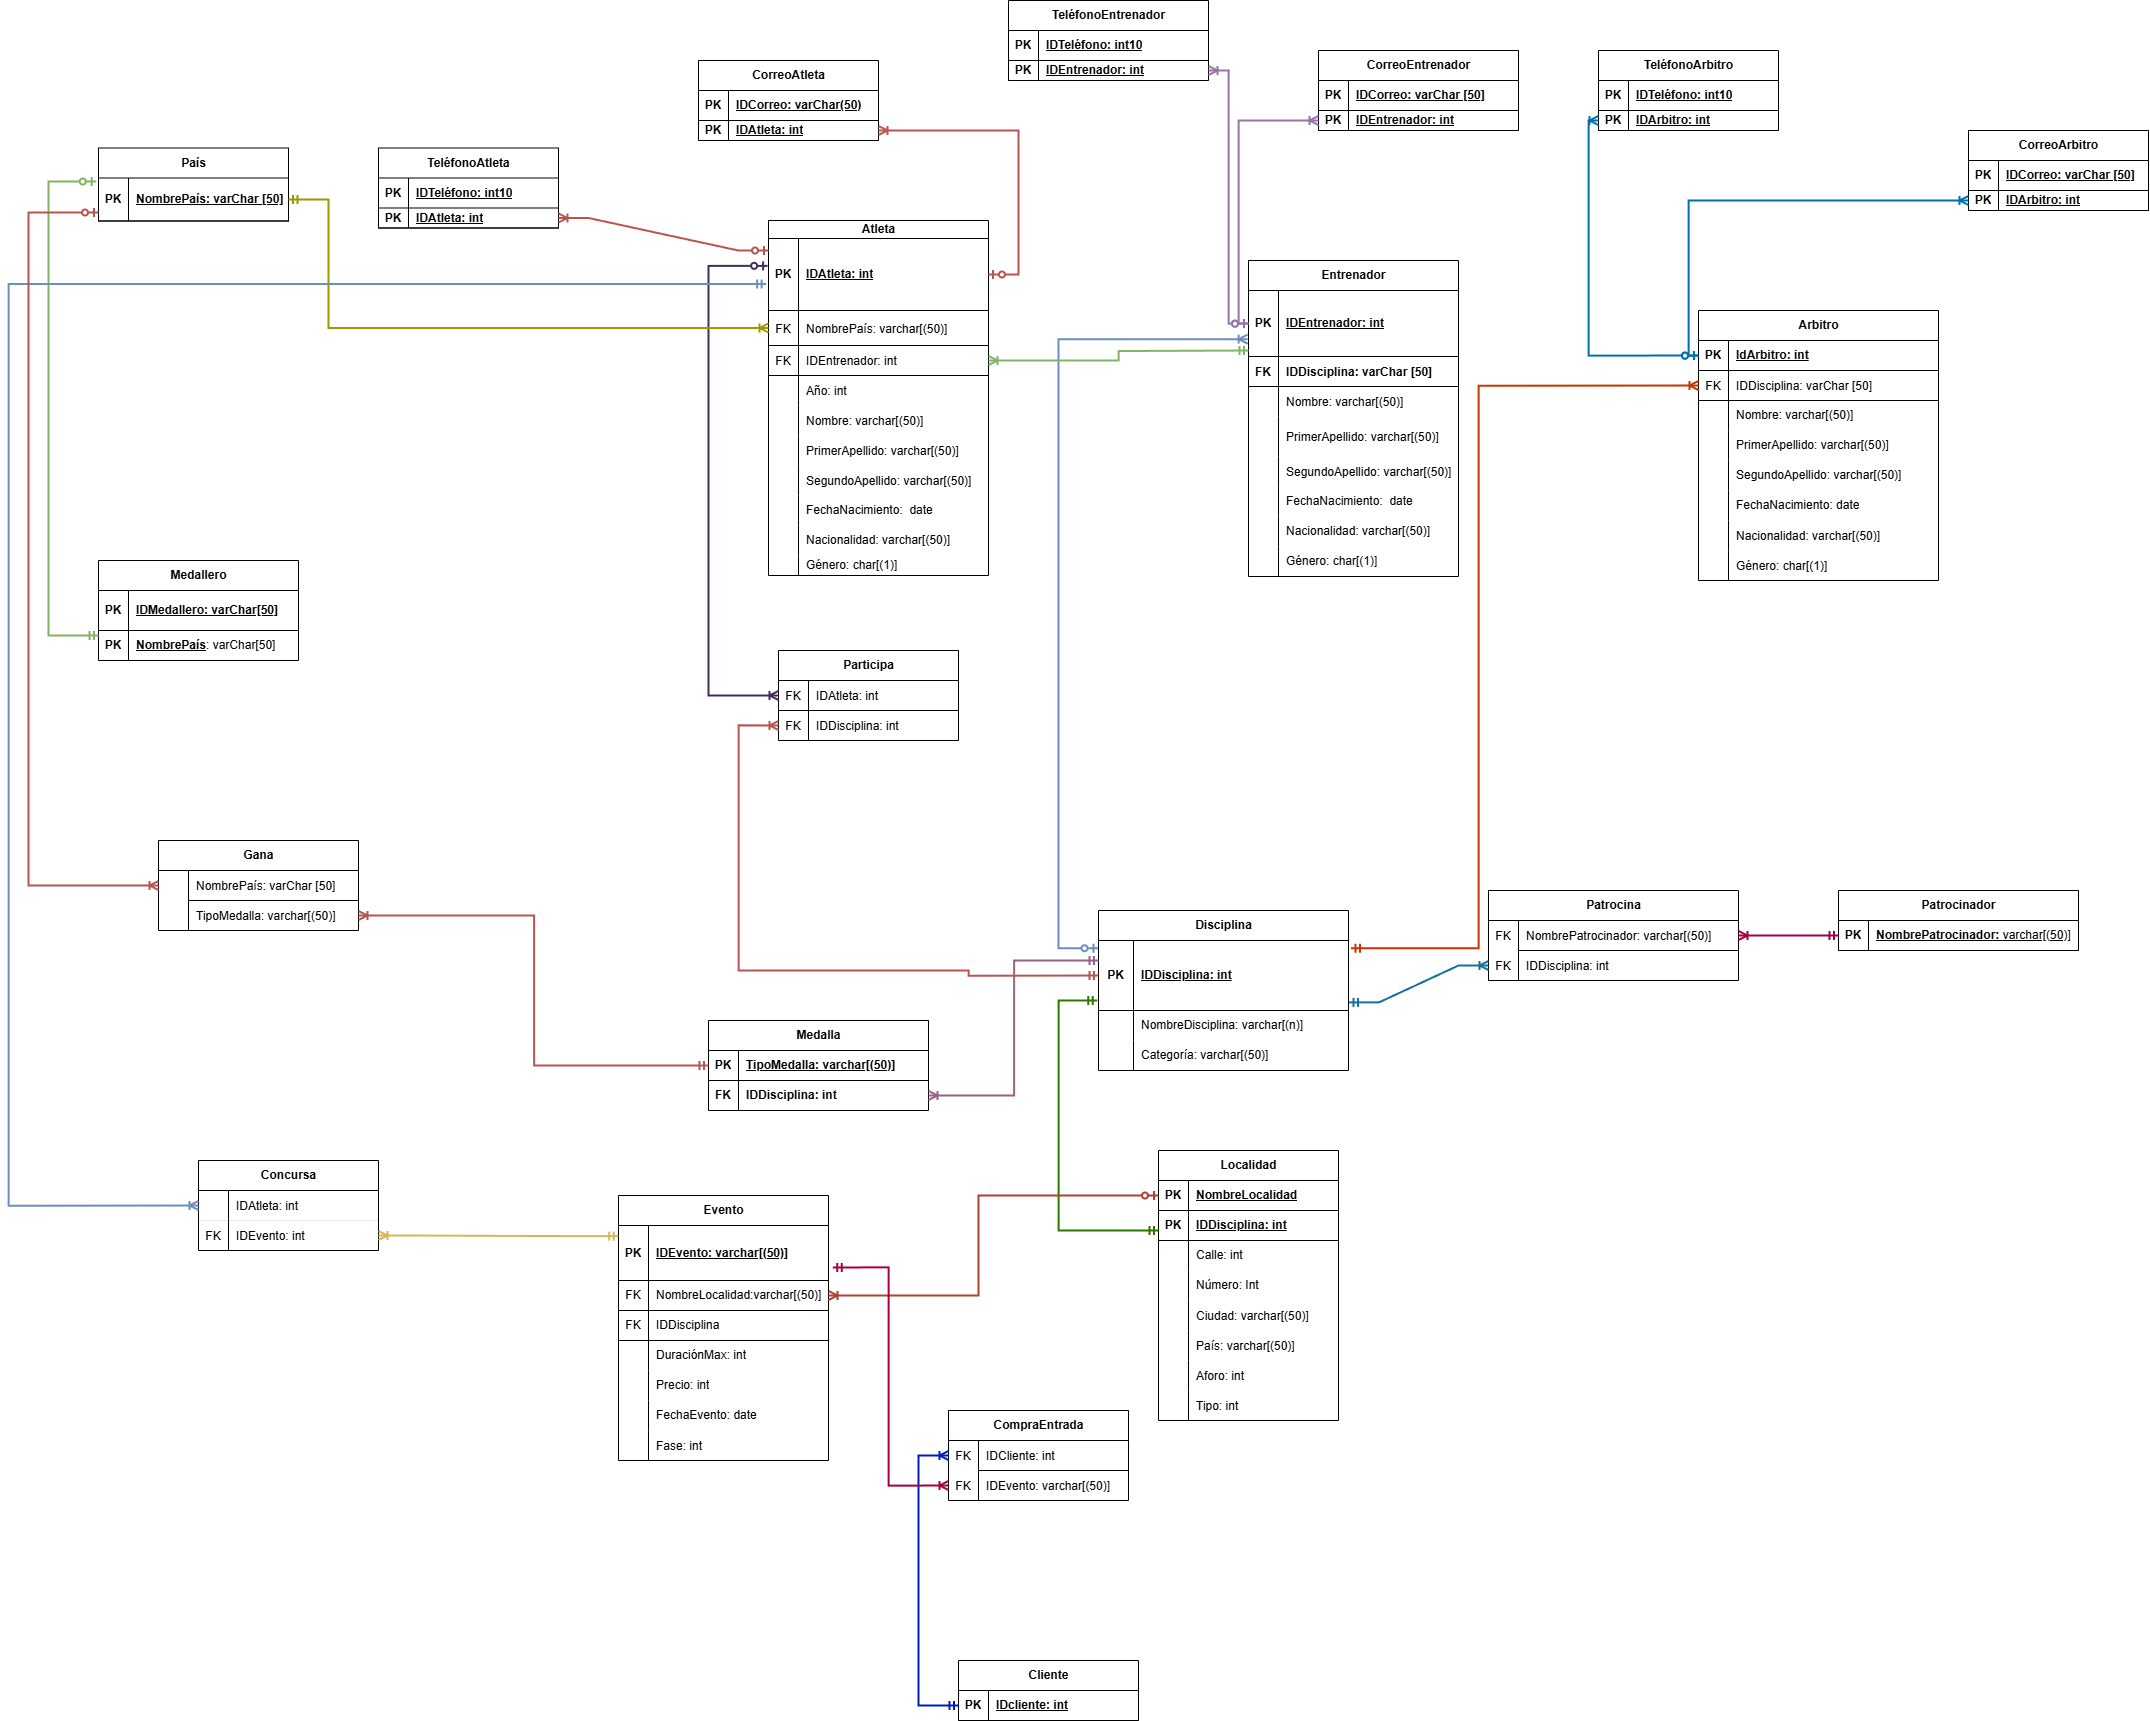
\includegraphics[width=1.1\textwidth]{resources/Modelo_Relacional.png}
    \caption{Modelo Relacional Práctica 4}
\end{figure}

\clearpage

\section{Modelo Entidad Relación de la Práctica 4:}
\begin{figure}[h]
    \centering
    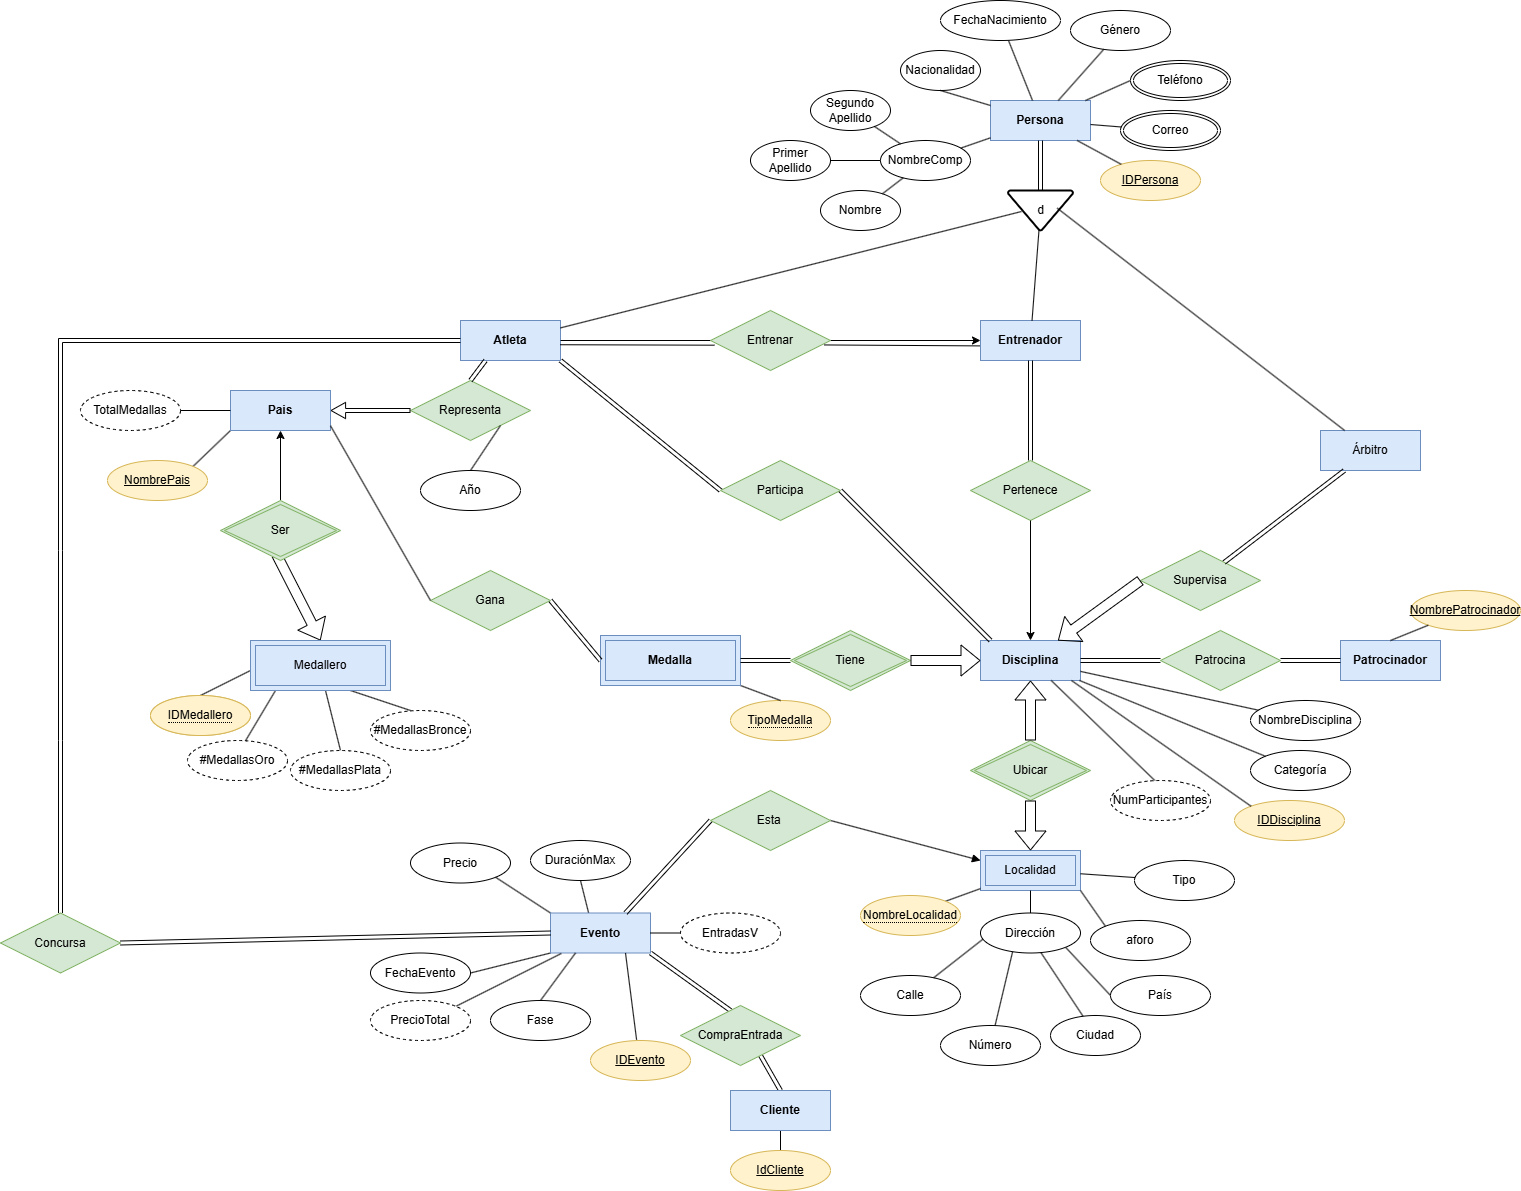
\includegraphics[width=1.1\textwidth]{resources/ModeloEntidad_Relación.png}
    \caption{Modelo Entida Relación Práctica 4}
\end{figure}

\clearpage

\section{Restauración del .backup}
\begin{figure}[h]
    \centering
    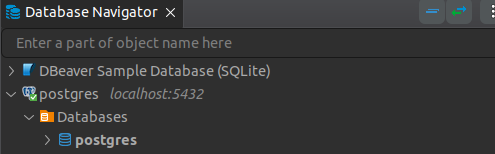
\includegraphics[width=1.1\textwidth]{resources/recovery/BD1.png}
    \caption{BD1}
\end{figure}

\begin{figure}[h]
    \centering
    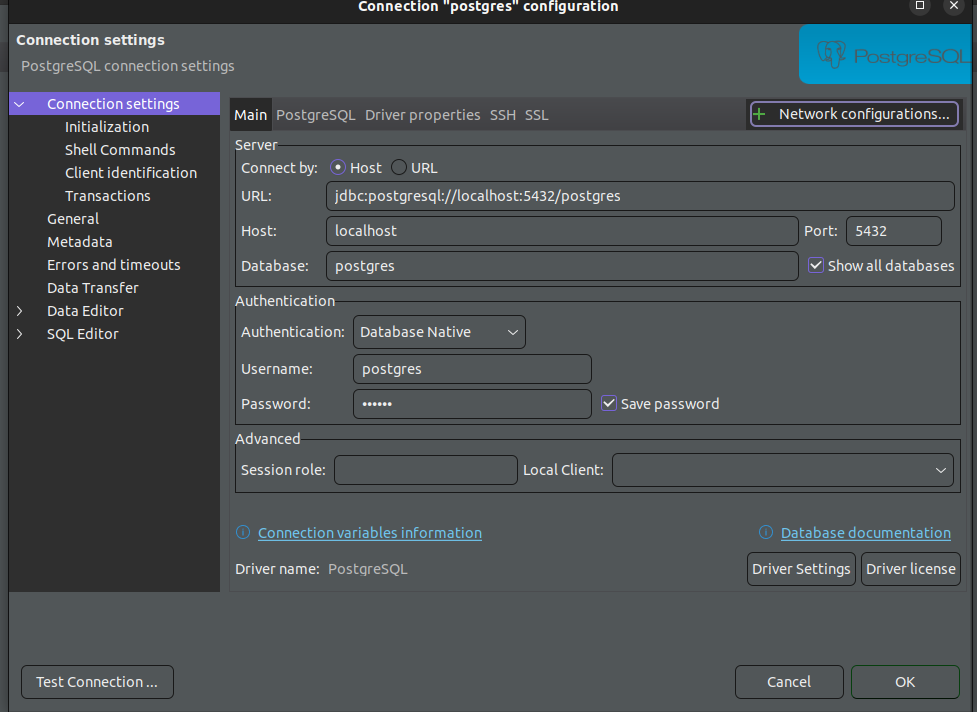
\includegraphics[width=1.1\textwidth]{resources/recovery/BD2.png}
    \caption{BD2}
\end{figure}

\begin{figure}[h]
    \centering
    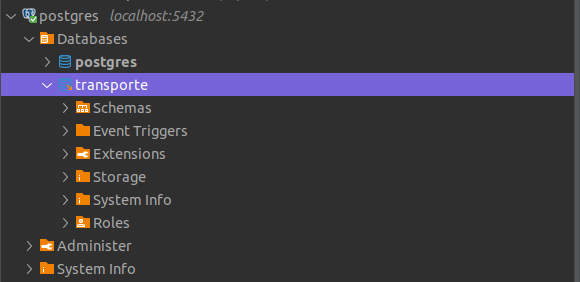
\includegraphics[width=1.1\textwidth]{resources/recovery/BD3.png}
    \caption{BD3}
\end{figure}

\begin{figure}[h]
    \centering
    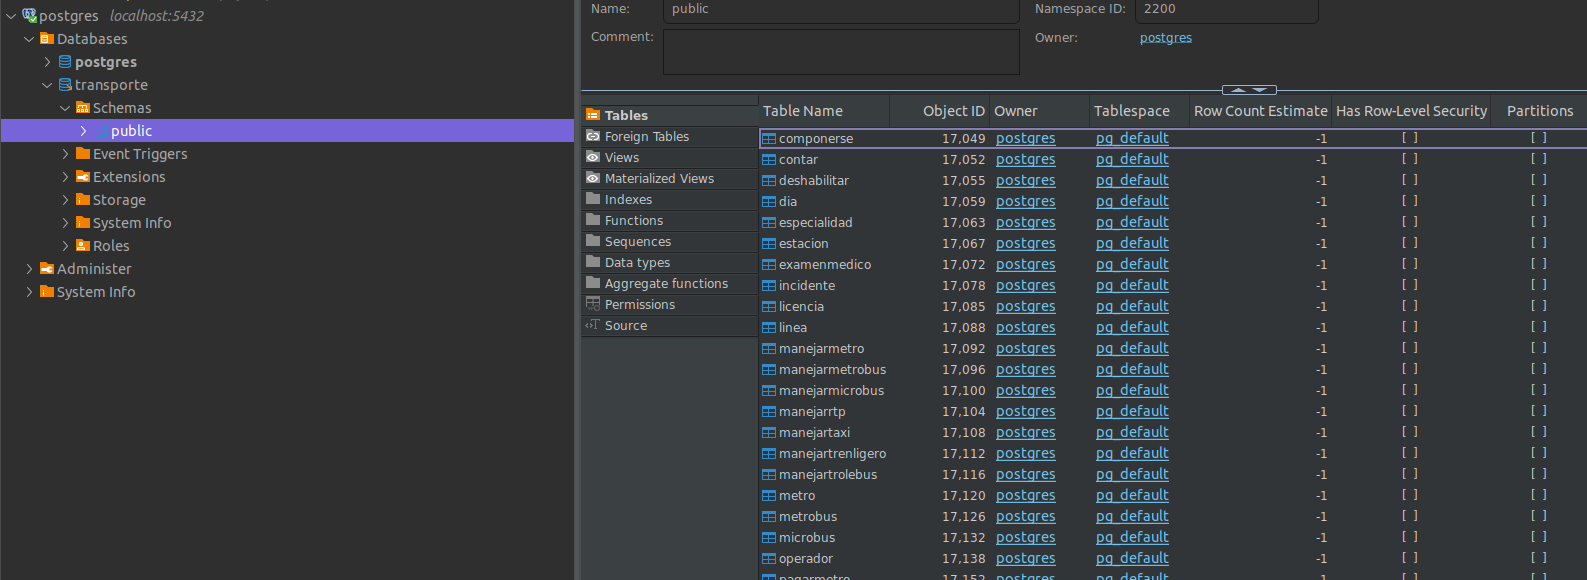
\includegraphics[width=1.1\textwidth]{resources/recovery/BD4.png}
    \caption{BD4}
\end{figure}

\begin{figure}[h]
    \centering
    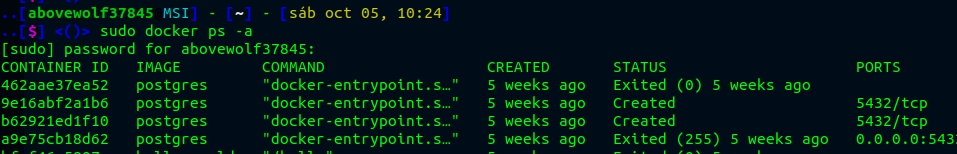
\includegraphics[width=1.1\textwidth]{resources/recovery/R1.png}
    \caption{R1}
\end{figure}

\begin{figure}[h]
    \centering
    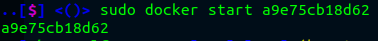
\includegraphics[width=1.1\textwidth]{resources/recovery/R2.png}
    \caption{R2}
\end{figure}

\begin{figure}[h]
    \centering
    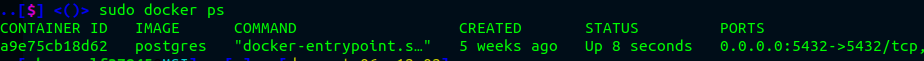
\includegraphics[width=1.1\textwidth]{resources/recovery/R3.png}
    \caption{R3}
\end{figure}

\begin{figure}[h]
    \centering
    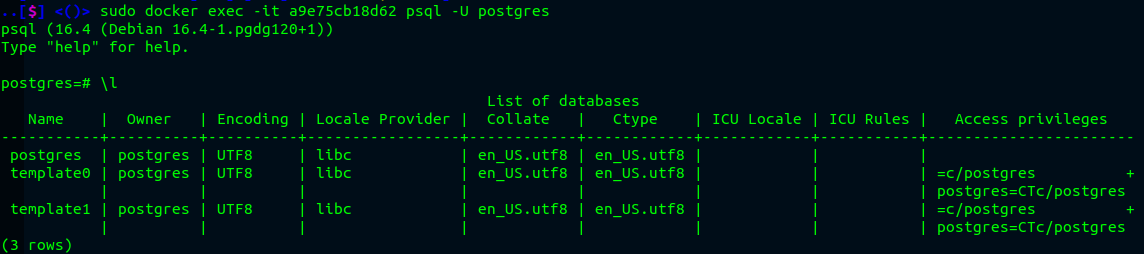
\includegraphics[width=1.1\textwidth]{resources/recovery/R4.png}
    \caption{R4}
\end{figure}

\begin{figure}[h]
    \centering
    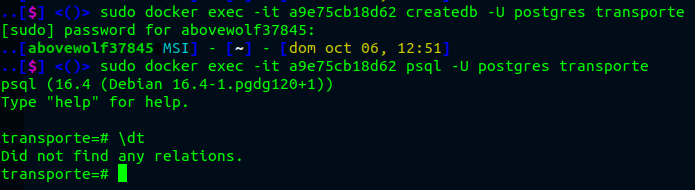
\includegraphics[width=1.1\textwidth]{resources/recovery/R5.png}
    \caption{R5}
\end{figure}

\begin{figure}[h]
    \centering
    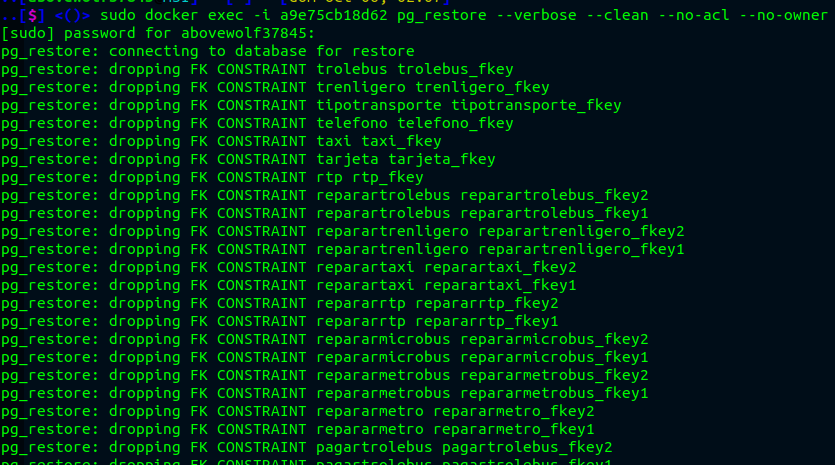
\includegraphics[width=1.1\textwidth]{resources/recovery/R6.png}
    \caption{R6}
\end{figure}

\begin{figure}[h]
    \centering
    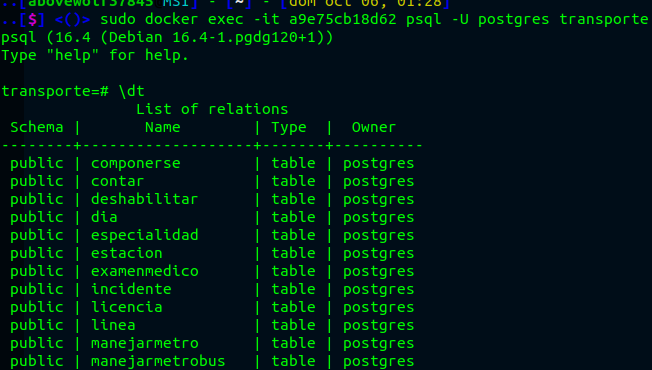
\includegraphics[width=1.1\textwidth]{resources/recovery/R7.png}
    \caption{R7}
\end{figure}

\clearpage

\section{Generación de la BDD}
\begin{figure}[h]
    \centering
    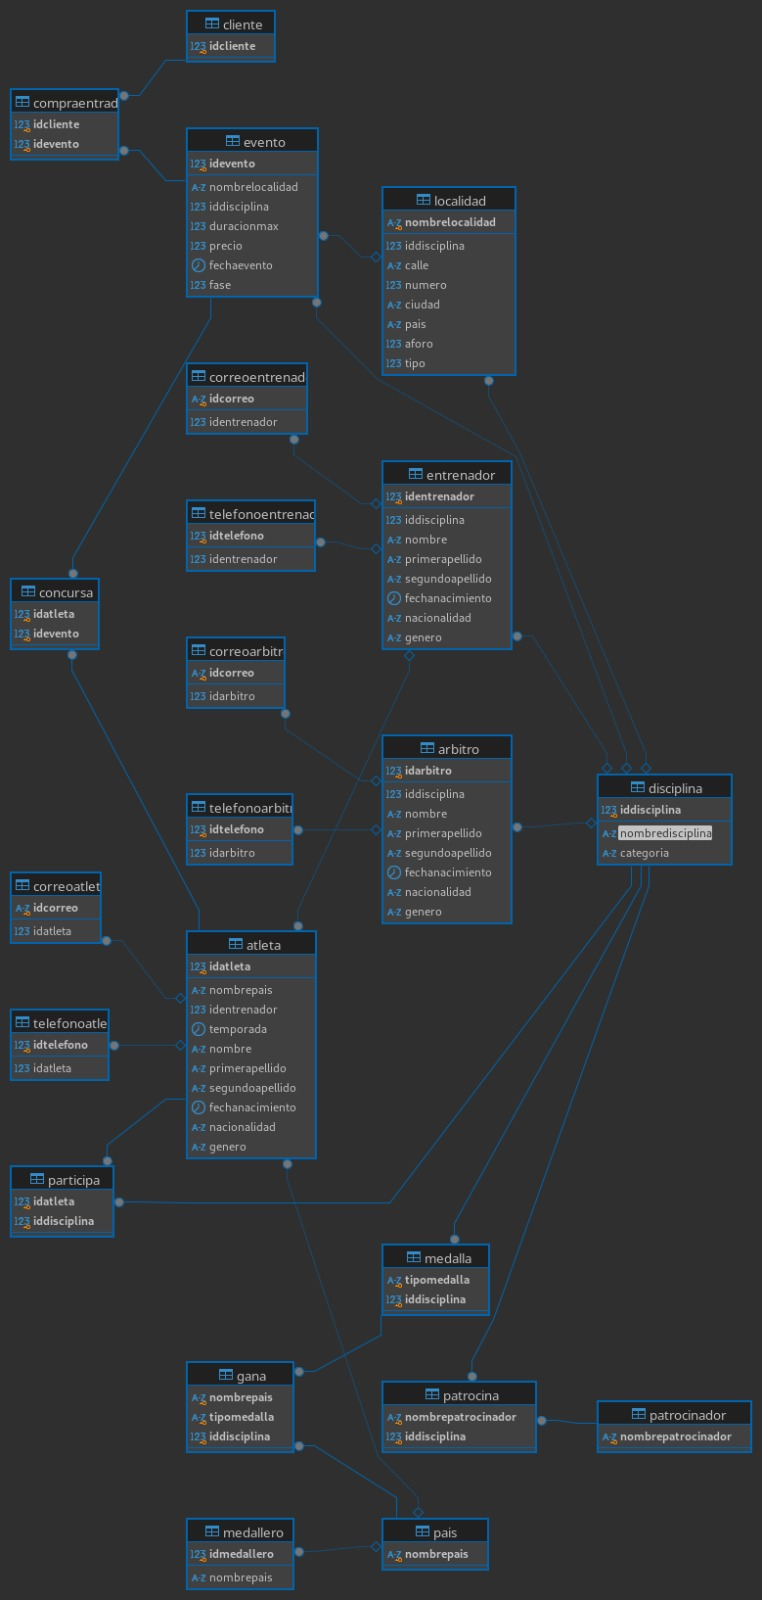
\includegraphics[width=.50\textwidth]{resources/Tablas.jpg}
    \caption{Generación de la BDD}
\end{figure}
